\chapter{Présentation - Tutoriel}



\section{Note de bas de page}

Exemple\footnotemark\\
%note en bas de page

\section{Glossaire et acronymes}

\gls{latex} is very useful and can use \gls{glsy}.

This tutorial which teach you glossary use from \acrlong{s2e}, which is  later abbreviated as \acrshort{s2e}  in this tutorial. This tutorial is useful for \acrlong{b2e}.


\section{Insérer une image}

%inclusion d'une image dans le document
\begin{figure}[!ht]
\begin{center}
% taille de l'image en largeur
% remplacer "width" par "height" pour régler la hauteur
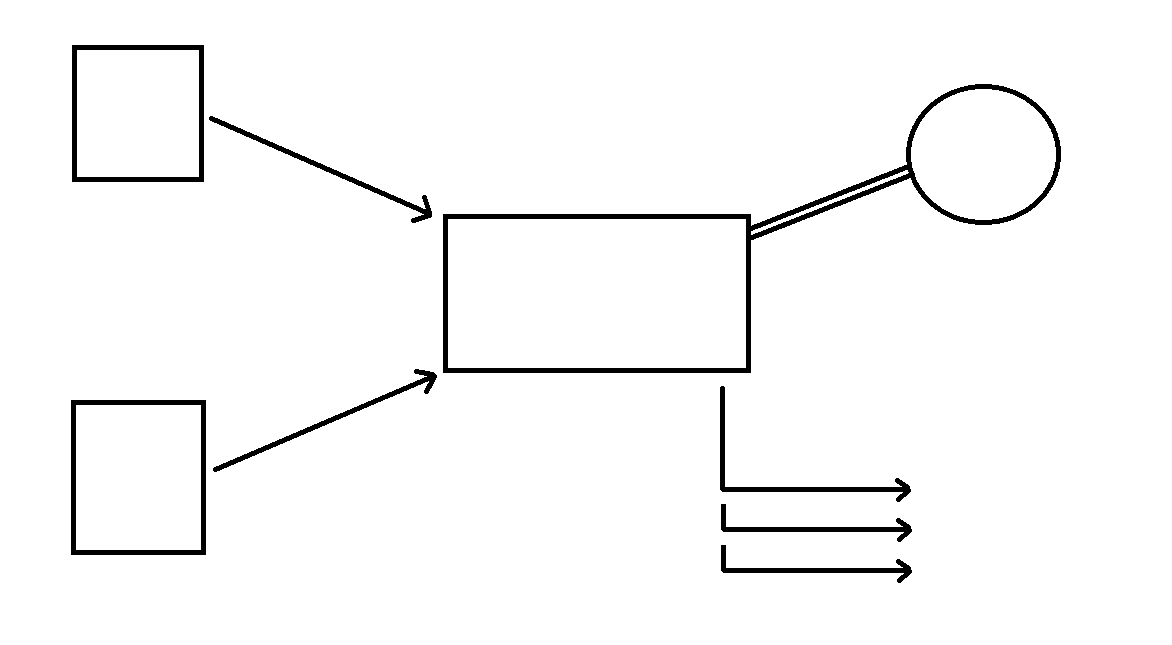
\includegraphics[width=15cm]{presentation/schema}
\end{center}
%légende de l'image
\caption{Schéma descriptif}
\end{figure}

\section{Galerie d'images}

%galerie d'image
\begin{figure}[htp]
  \centering
  \subfloat[Première image]{\label{fig:première}
\includegraphics[scale=0.7]{resultats/gallerie}}
  ~ %espace entre deux images sur une même ligne
  \subfloat[Deuxième image]{\label{fig:deuxième}
\includegraphics[scale=0.7]{resultats/gallerie}}
  ~
  \subfloat[Troisième image]{\label{fig:troisième}
\includegraphics[scale=0.7]{resultats/gallerie}}
  ~\\ %saute une ligne dans la galerie d'image
  \subfloat[Quatrième image]{\label{fig:quatrième}
\includegraphics[scale=0.7]{resultats/gallerie}}
  ~
  \subfloat[Cinquième image]{\label{fig:cinquième}
\includegraphics[scale=0.7]{resultats/gallerie}}
  \caption{Différents screenshots quelque chose, en galerie}
  \label{fig:gallerie1}
\end{figure}

\newpage
\section{Insérer un tableau}
%tableau centré à taille variable qui s'ajuste automatiquement suivant la longueur du contenu

\begin{figure}[!ht]
\begin{center}
\begin{tabular}{|l|l|l|l|l|}
  \hline
  Solution & Critère 1 & Critère 2 & Critère 3 & Critère 4\\
  \hline
  Solution 1(cf. ref. \cite{vaughnShaderResources2021}) & Oui & Oui & Oui & Oui \\
  Solution 2(cf. ref. \cite{vaughnShaderResources2021}) & Oui & Oui & Oui & Non \\
  Solution 3(cf. ref. \cite{vaughnShaderResources2021}) & Oui (sauf telle chose) & Non & Non & Oui\\
  Solution 4(cf. ref. \cite{vaughnShaderResources2021}) & Oui& Non & Oui & Non\\
  Solution 5(cf. ref. \cite{vaughnShaderResources2021}) & Oui (uniquement ceux-ci) & Non & Oui & Non\\
  \hline
\end{tabular}
\end{center}
\caption{Tableau récapitulatif des solutions}
\end{figure}


%Contenu de la note précédemment marquée avec \footnotemark
\footnotetext{Note bas de page "intro"}

\newpage

\section{Centrer du texte}

\begin{center}
Problématique du sujet
\end{center}

\section{Listes}


Voici une liste :
\begin{itemize}
\item item 1;
\item item 2;
\item item 3;
\item item 4.
\end{itemize}


\section{Citation biblio}


%Detail :
Bla(cf. ref. \cite{vaughnShaderResources2021}).
%citation référencé dans le document "bibliographie.bib" inclus à la fin du document

\footnotetext{Note bas de page "bla"}